\documentclass[border=1mm]{standalone}
\usepackage{tikz}
\usepackage{circuitikz}
\usetikzlibrary{arrows,shapes.gates.logic.US,shapes.gates.logic.IEC,calc}

\begin{document}
	\thispagestyle{empty}
	\tikzstyle{branch}=[fill,shape=circle,minimum size=3pt,inner sep=0pt]
	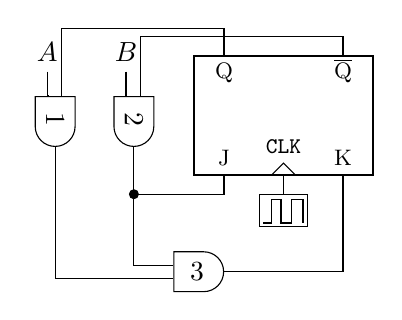
\begin{tikzpicture}[label distance=2mm]
	\node (A) at (0,0) {$A$};
	\node (B) at (1,0) {$B$};
\node[and gate US, draw, logic gate inputs=nn,rotate=-90,anchor=output] at ($(A)+(0.1,-1.2)$) (gate1) {1};
\node[and gate US, draw, logic gate inputs=nn,rotate=-90,anchor=output] at ($(B)+(0.1,-1.2)$) (gate2) {2};
\node[and gate US, draw, logic gate inputs=nn, anchor=input 1] at ($(gate2.output)+(0.5,-1.5)$) (gate3) {3};
\draw (A) |- (gate1.input 2);
\draw (B) |- (gate2.input 2);

\draw (3,-0.8) node[flipflop JK, rotate=90, scale=0.9, flipflop def={t2={\texttt{CLK}}}](ff1){};

\draw (gate1.input 1) |- ([yshift=0.1cm]ff1.pin 6) -- (ff1.pin 6); % Q
\draw (gate2.input 1) |- (ff1.pin 4); % Qn
\draw (gate1.output) |- (gate3.input 2);
\draw (gate2.output) |- (gate3.input 1);

\draw (ff1.pin 3) |- (gate3.output);
%\draw (gate1.output)  to[short, -*] ([yshift=-0.6cm]gate1.output) node[above] {} |- (ff1.pin 1);
\draw (gate2.output)  to[short, -*] ([yshift=-0.6cm]gate2.output) node[above] {} |- (ff1.pin 1);

% Clock
\node[draw, minimum width=0.6cm, minimum height=0.4cm](CLK) at ([yshift=-0.2cm]ff1.pin 2) {};
\draw (CLK.south west) ++(0.05,0.05) -| ++(0.1,0.3) -| ++(0.125,-0.3) -| ++(0.135,0.3) -| ++(0.145,-0.3);

 	\end{tikzpicture}
\end{document}
